\documentclass[12pt]{article}
\usepackage{algorithmicx}
\usepackage[ruled]{algorithm}
\usepackage{algpseudocode}
\usepackage{algpascal}
\usepackage{algc}
\usepackage{url,enumerate, amssymb, anysize, booktabs, amsfonts}
\usepackage[colorlinks = true,
linkcolor = blue,
urlcolor  = blue,
citecolor = green,
anchorcolor = blue]{hyperref}
\usepackage{setspace,listings}
\usepackage[dvipdfmx]{graphicx}
\usepackage{amsmath}
\usepackage{psfrag}
\usepackage[font=small,labelfont=bf]{caption}
\usepackage{enumerate}
\usepackage{natbib}
\usepackage{url} % not crucial - just used below for the URL 


\begin{document}
	
	\title{Testing independence between networks and nodal attributes via multiscale metrics}
	
	\author{Youjin Lee}
	
	\maketitle
		
%%%%%%%%%%%%%%%%%%%%%%%%%%%%%%%%%	
\subsection*{1. Introducing network topology}

\begin{figure}[H]
	\centering
	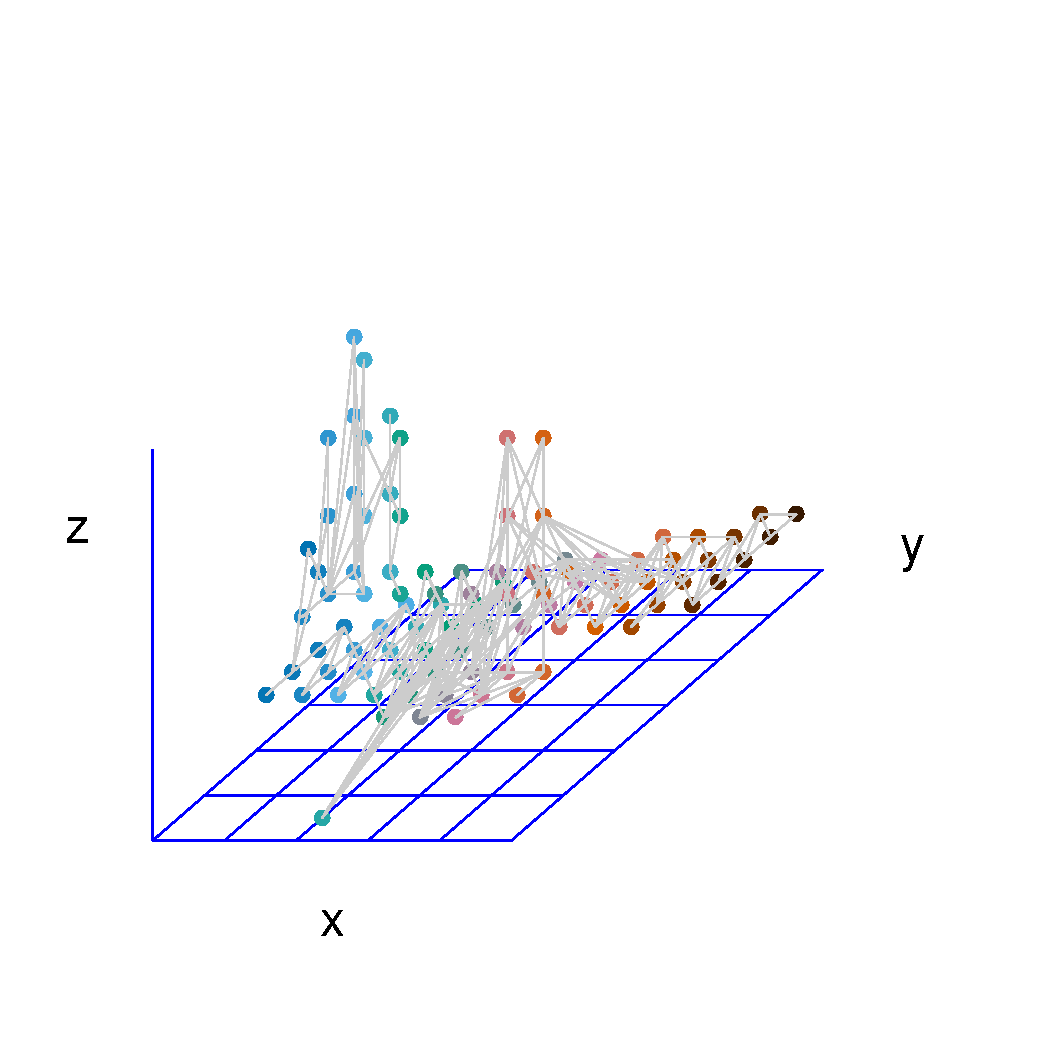
\includegraphics[width=3in]{../Figure/intro.pdf}	
	\label{fig:intro}
\end{figure}

You can embed each subject (node) connected via edges upon Euclidean space, e.g. $xyz$ 3D-space as above, according to their possessing attributes, e.g. physical location; while how to embed subjects from network into Euclidean space is not intuitive, which should consider their distance with respect to network relationship.

\subsection*{2. Problems in adopting  valid distance metric defined over network}

\begin{figure}[H]
	\centering
	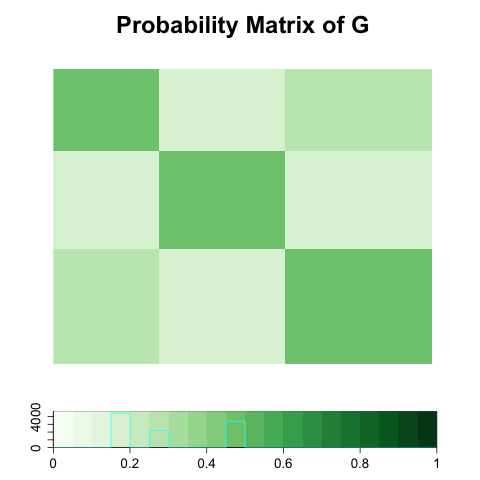
\includegraphics[width=1.5in]{../Figure/pmat.png}
	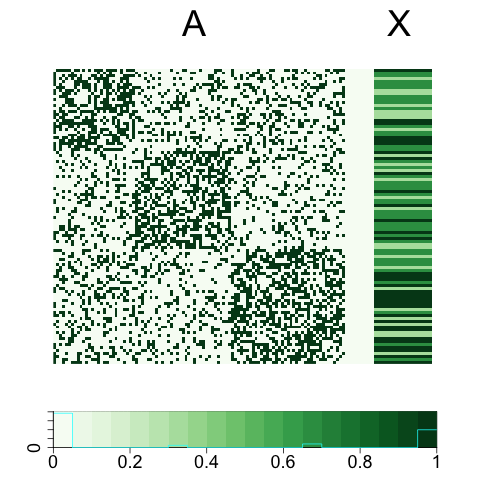
\includegraphics[width=1.5in]{../Figure/Amat.png}
	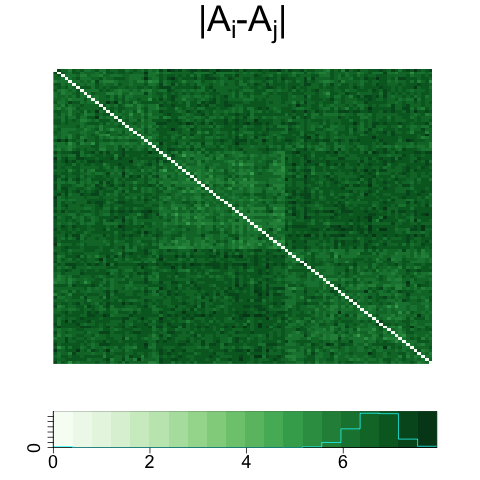
\includegraphics[width=1.5in]{../Figure/distA.png}
	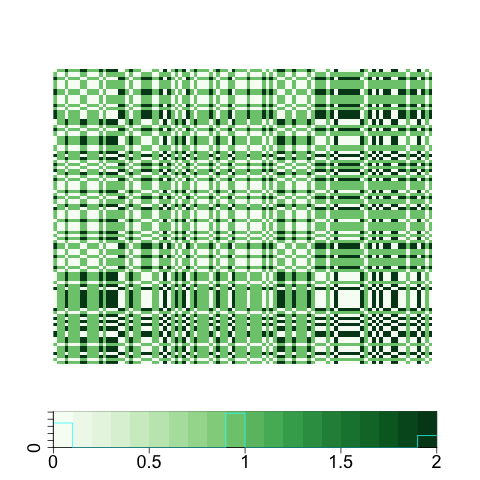
\includegraphics[width=1.5in]{../Figure/distX.png}
	\label{fig:matrics}
\end{figure}	

Assuming that a set of edges $\{ A \}$ are distributed following certain stochastic block model, also depending on the distribution function of nodal attributes $X$(a), then with some amount of noise we have a realized adjacency matrix and a set of attribute outcomes(b) of which Euclidean distances (c)(d) are constructed to be possibly used in standard distance-based independence test.

\subsection*{3. introduce a family of network distance matrices} 

\begin{figure}[H]
	\centering
	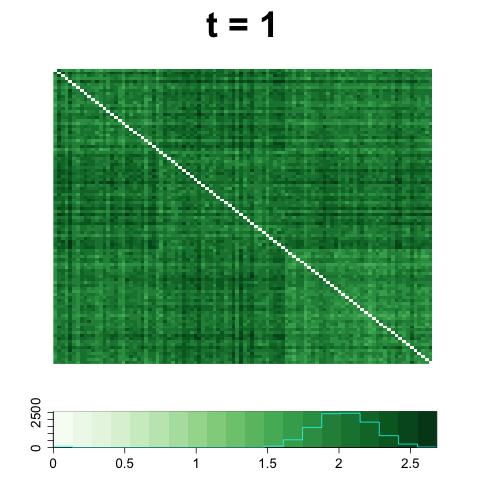
\includegraphics[width=1.5in]{../Figure/Dx1.png}
	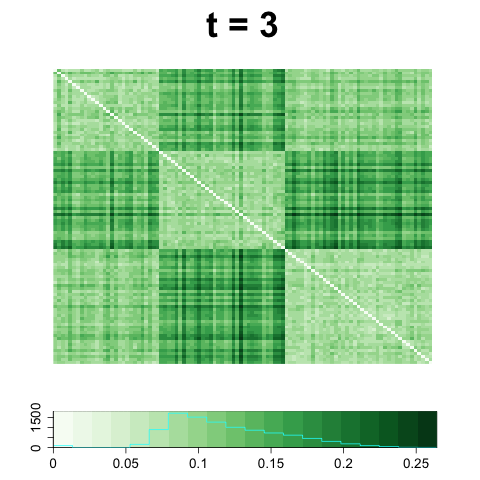
\includegraphics[width=1.5in]{../Figure/Dx3.png}
	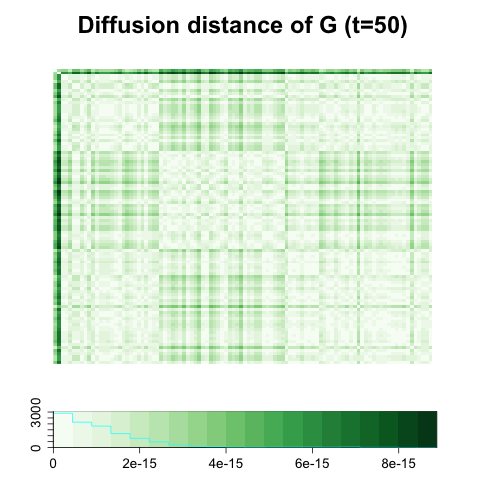
\includegraphics[width=1.5in]{../Figure/Dx50.png}
	\label{fig:diffusions}
\end{figure}	

\textit{Diffusion matrix}, as a proper alternative for Euclidean distance of $A$, provides one-parameter family of network-based distance where at early stage, e.g. at $t=1$, distance matrix is very similar to Euclidean distance of $A$ by taking into account very close relationship but as time goes by the pattern shown in the distance matrix changes, depending on time $(t)$ spent on diffusion process. 

\subsection*{4. Empirical power of Oracle MGC/Sample MGC}

\begin{figure}[H]
	\centering
	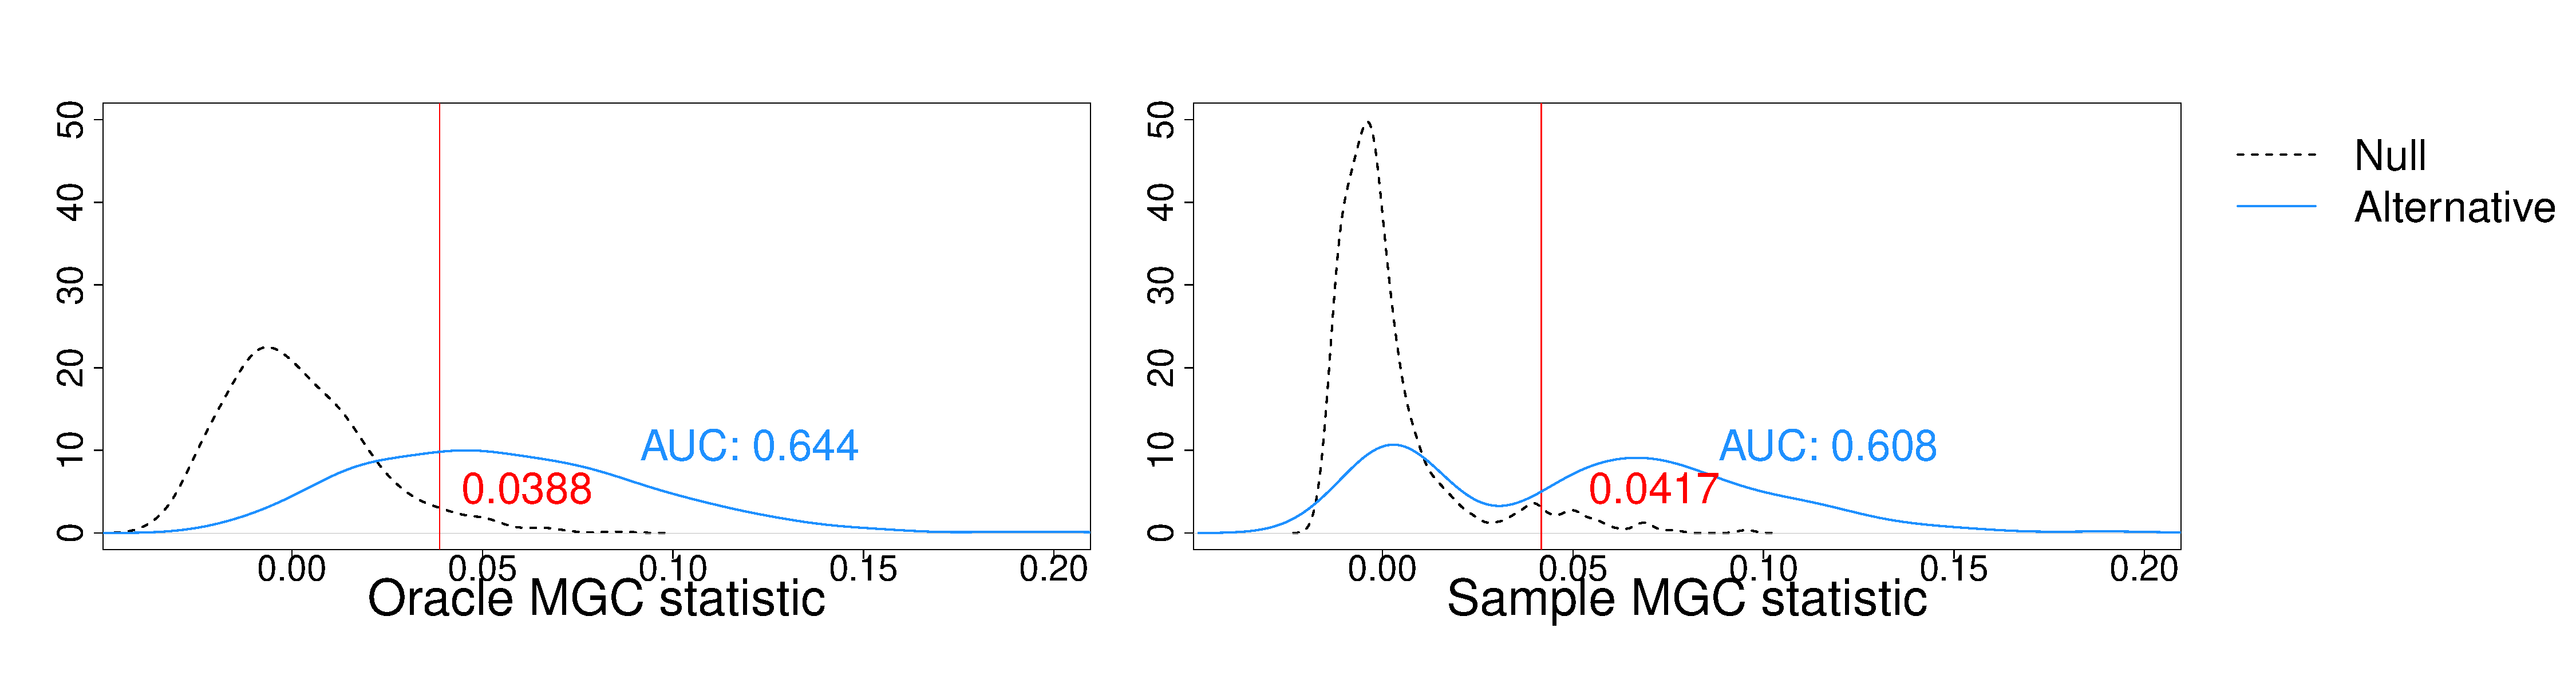
\includegraphics[width=6in]{../Figure/density.pdf}
	\label{fig:density}
\end{figure}	
 
In the left panel we have empirical Null distribution of \texttt{Oracle MGC} illustrated by black line of which 95$\%$ sample quantile determines testing power of \texttt{Oracle MGC} by calculating area under the curve (AUC) of the empirical distribution under alternative beyond that quantile, and AUC of \texttt{Oracle MGC} (0.644) looks similar to that of \texttt{Sample MGC} (0.608), as presented in the right panel, even though the shape of its distributions under null and alternative look different, which supports the use of \texttt{Sample MGC} as a substitute for \texttt{Oracle MGC} in real data.
 
\subsection*{5. Simplest Stochastic Block Model}
 
\begin{figure}[h]
	\centering
	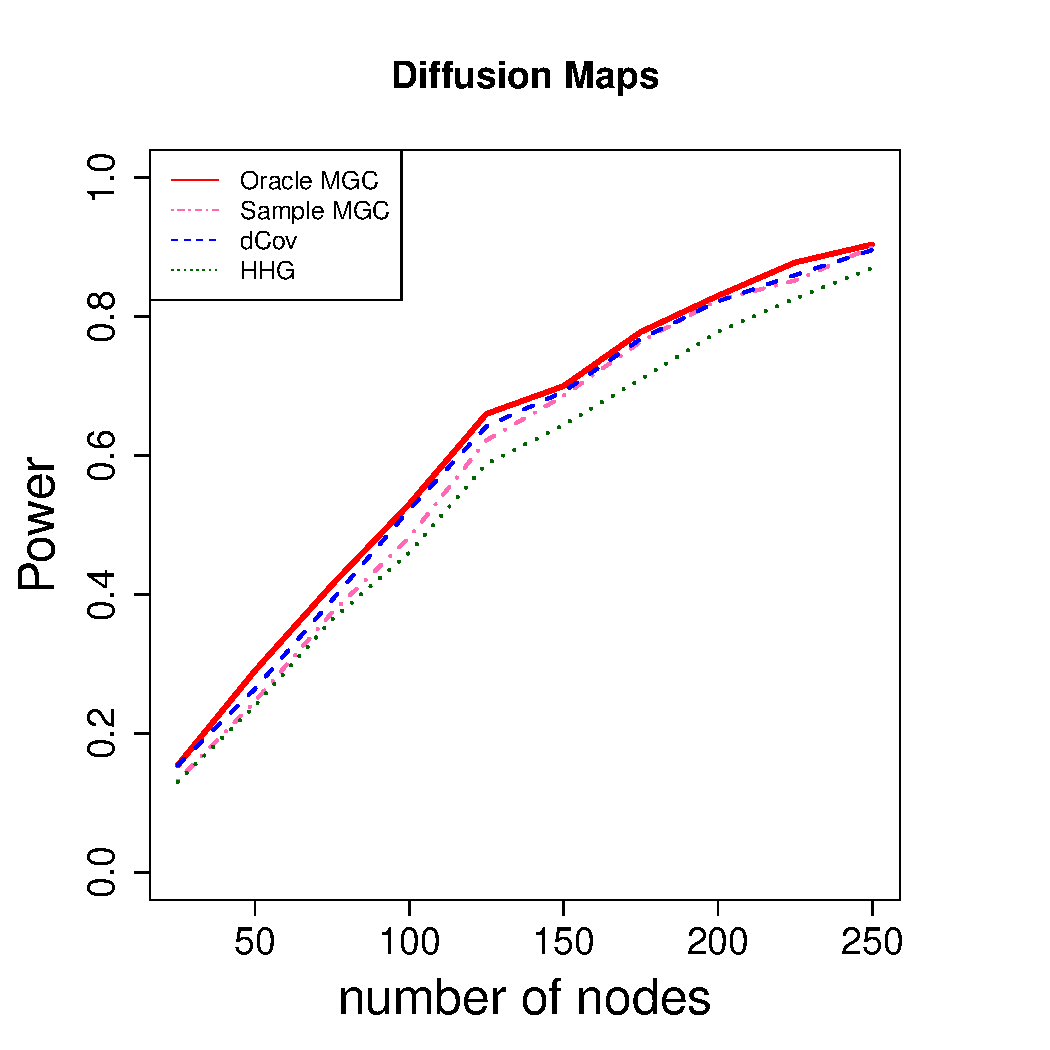
\includegraphics[width=6in]{../Figure/twoSBM.pdf}
	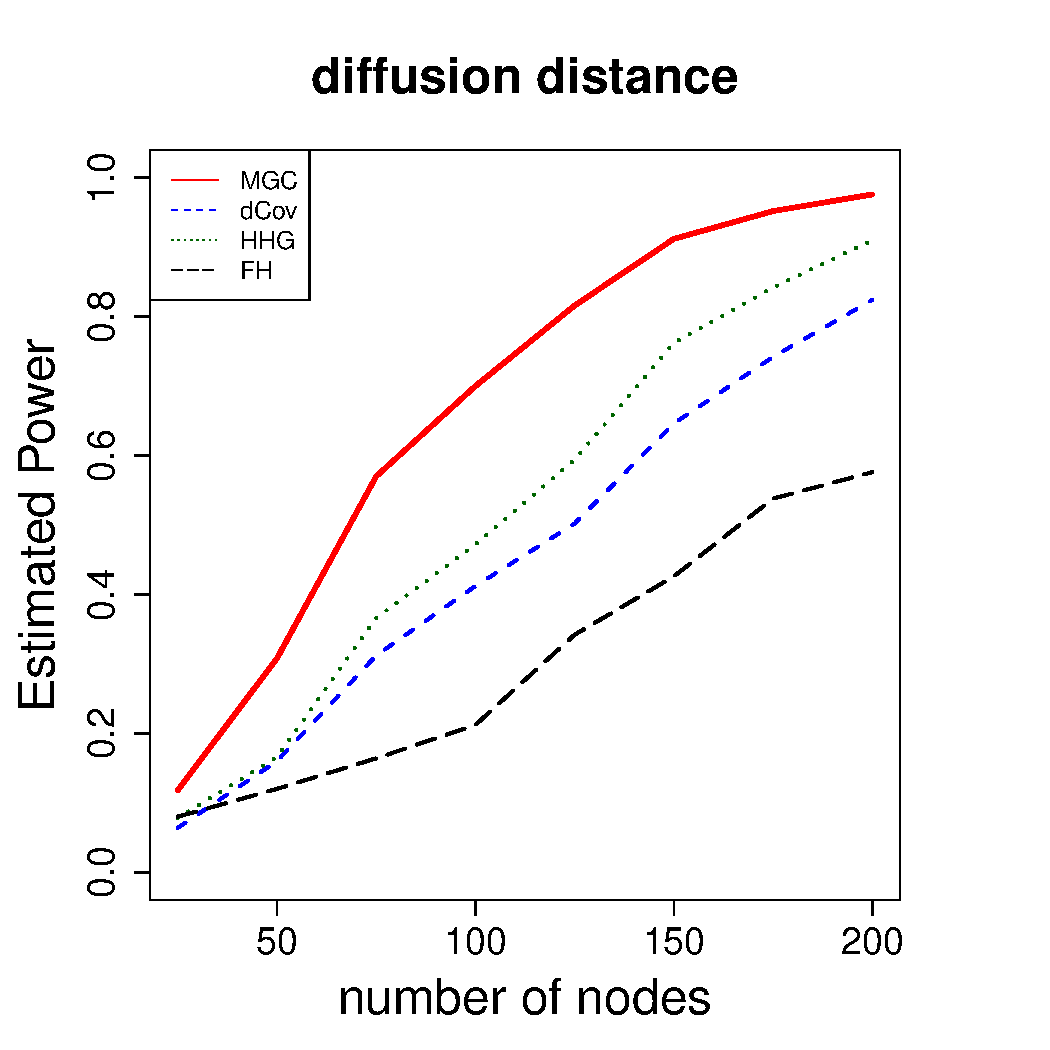
\includegraphics[width=6in]{../Figure/ThreeSBM.pdf}
\end{figure}

Top three figures are showing power of network independence test  under two block SBM using diffusion maps, adjacency matrix, and estimated latent position as a network distance measure where results based on three metrics are similar as well as \texttt{MGC}, global distance-based tests (\texttt{dCov, HHG}) and \texttt{FH} tests are; whereas under three block SBM diffusion maps generally perform better than the other metrics across all type of distance-based tests and moreover \texttt{FH} test results worse than the others even in the metrics of latent position.

\subsection*{6. Superiority of the proposed method under non-linear dependency}

\begin{figure}[H]
	\centering
	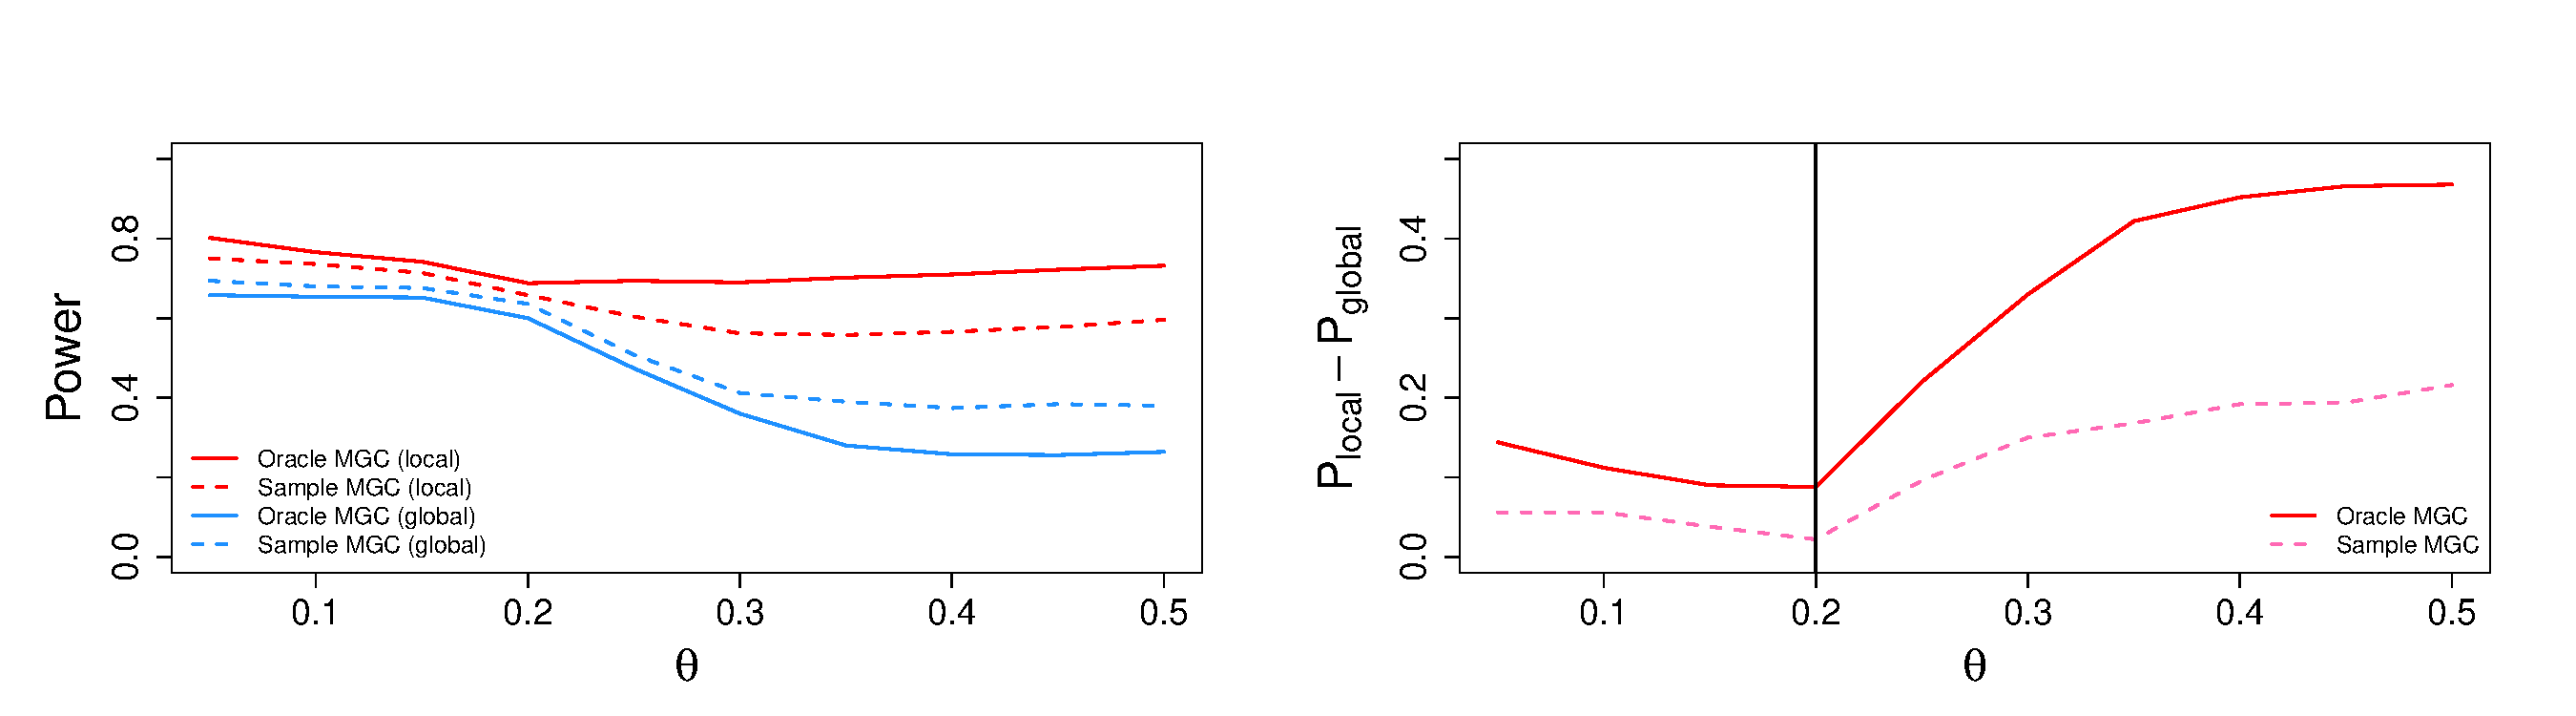
\includegraphics[width=5in]{../Figure/powerplot.pdf}
	\label{fig:powerplot}
\end{figure}

A x-axis of $\theta$ controls the existence/amount of non-linear dependency and in this particular case non-linearity exists when $\theta > 0.2$ and gets larger as it increases, and you can see the discrepancy in power between global and local scale tests also gets larger accordingly, mostly due to decreasing power of global test under non-linear dependency as presented in the left panel.

\subsection*{7. Degree-corrected SBM with increased variability in node distribution}	

\begin{figure}[H]
	\centering
	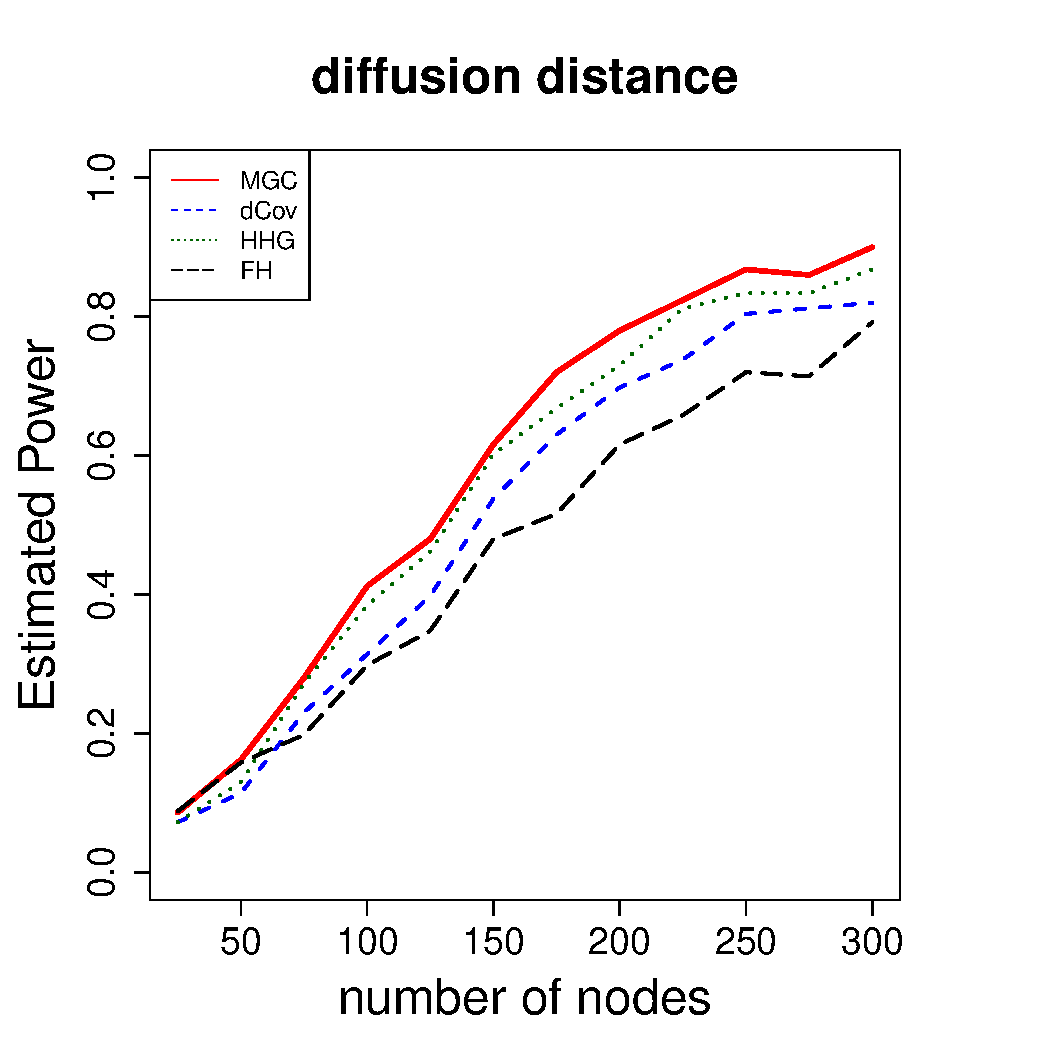
\includegraphics[width=6in]{../Figure/dcSBM.pdf}
	\label{fig:dcSBM}
\end{figure}	

In DCSBM, the performance of all distance-based tests under distance maps used are similar but under adjacency matrix metric, global distance-based tests fail to detect the dependency due to an increased variability in $A$, which also possibly explains why \texttt{FH} outperforms the others under also more variable latent position metric.


\subsection*{8. Validity of the method even under competitor's model}

\begin{figure}[H]
	\centering
	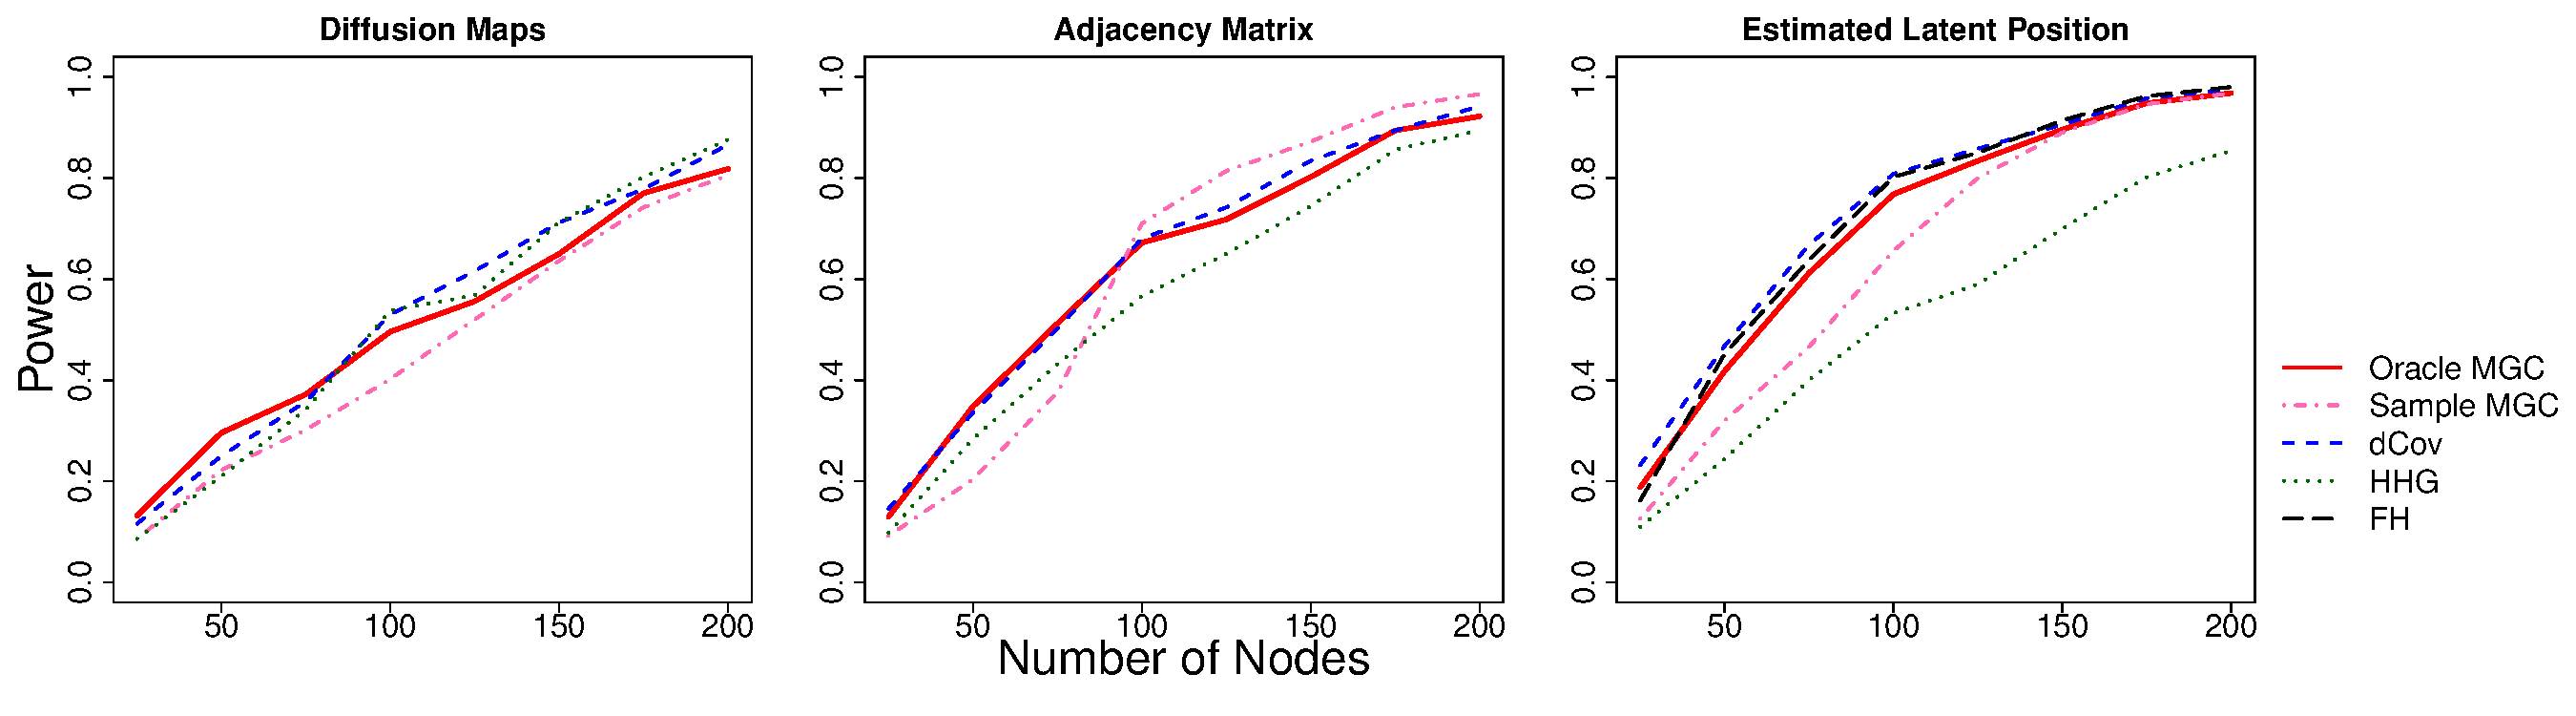
\includegraphics[width=6in]{../Figure/ame.pdf}
	\label{fig:ame}
\end{figure}	

Under additive and multiplicative model, where no specific test methods beat the others significantly, estimated latent positions provide most sensitive power for \texttt{MGC} and \texttt{FH}, and they result similar power even though this model is deliberately designed to favor \texttt{FH} tests.

\subsection*{9. Node Contribution}

\begin{figure}[H]
	\centering
	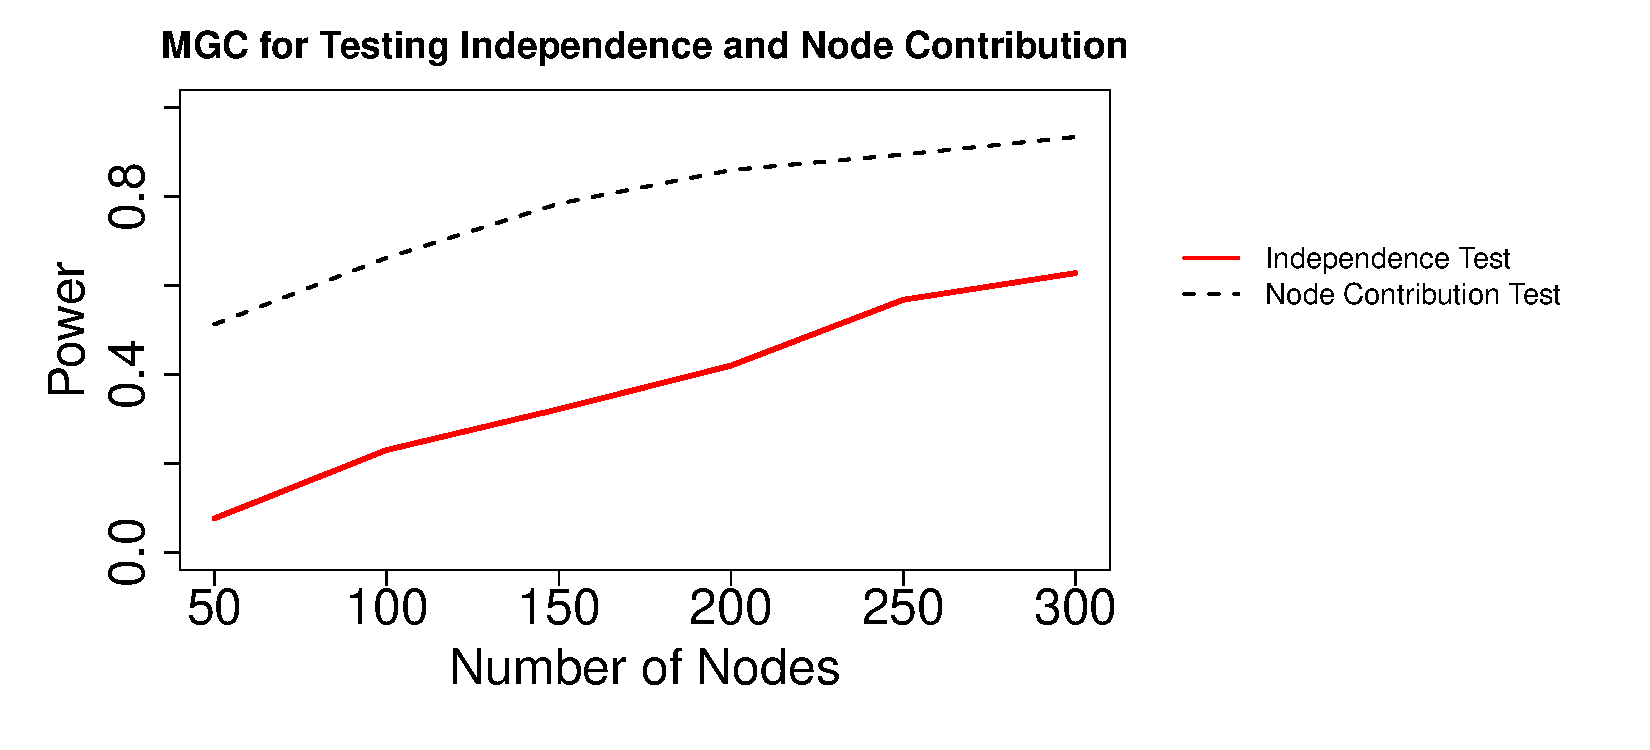
\includegraphics[width=6in]{../Figure/nodecontri.pdf}
	\label{fig:contribution}
\end{figure}

This plot describes both power of \texttt{MGC} and the rate of correctly-ranked node contribution increase as the number of nodes increases when only half of the nodes for each simulation actually are set to contribute to the independence test. 


\end{document}